% Template:     Auxiliar LaTeX
% Documento:    Archivo principal
% Versión:      8.3.3 (20/01/2025)
% Codificación: UTF-8
%
% Autor: Pablo Pizarro R.
%        pablo@ppizarror.com
%
% Manual template: [https://latex.ppizarror.com/auxiliares]
% Licencia MIT:    [https://opensource.org/licenses/MIT]

% CREACIÓN DEL DOCUMENTO
\documentclass[
	spanish, % Idioma: spanish, english, etc.
	letterpaper, oneside
]{article}

% INFORMACIÓN DEL DOCUMENTO
\def\documenttitle {Auxiliar 6}
\def\documentsubject {Dinámica}

\def\documentauthor {Nombre del autor}
\def\coursename {Mecánica}
\def\coursecode {FI-2001}

\def\universityname {Universidad de Chile}
\def\universityfaculty {Facultad de Ciencias Físicas y Matemáticas}
\def\universitydepartment {Departamento de la Física}
\def\universitydepartmentimage {departamentos/fcfm}
\def\universitydepartmentimagecfg {height=1.75cm}
\def\universitylocation {Santiago de Chile}

% EQUIPO DOCENTE
\def\teachingstaff {
	\textbf{Profesor: Simón Riquelme} \\
	Auxiliares: Jorge Barja, Ian Tobar \\
	Ayudante: Matías Abrigo  \\
}

% IMPORTACIÓN DEL TEMPLATE
\input{template}

% INICIO DE PÁGINAS
\begin{document}

% CONFIGURACIÓN DE PÁGINA Y ENCABEZADOS
\templatePagecfg

% ======================= INICIO DEL DOCUMENTO =======================

\newboxquestion{P1}\\

--++++Considere una bolita de masa $m$ ensartada en una barra de manera que puede deslizar sin roce por ella. La masa está atada mediante un resorte, de constante elástica $k$ y largo natural $l_0$, a un extremo de la barra, y esta última, a su vez, gira c/r al mismo extremo en un plano horizontal con velocidad angular $w$ constante. En $t=0$ la bolita se suelta con resorte comprimido en $l_0/2$ y $\dot{\rho}(0) = 0$:

\begin{enumerate}[label=\alph*)]
    \item ¿Qué relación deben cumplir $m,k$ y $w$ para que la bolita realice un movimiento armónico simple a lo largo de la barra?.
    \item Determine la compresión del resorte como función del tiempo..

\end{enumerate}


% \begin{figure}[ht] % [h] indica que se coloca la imagen aquí (here)
%     \centering % Centra la imagen
%     
\includegraphics[width=0.4\textwidth]{p1.png} % Ajusta el tamaño de la imagen
%     \caption{Pregunta 1.} % Subtítulo de la imagen
%     \label{fig:p1} % Etiqueta opcional para referencias
% \end{figure}

\begin{figure}[h]
    \centering
    % Primera imagen
    \begin{subfigure}[b]{0.4\textwidth}
        \centering
        
\includegraphics[width=\textwidth]{p1.png}
        \caption{Pregunta 1}
        \label{fig:imagen1_1}
    \end{subfigure}
    \hspace{0.5cm} % Espacio entre las imágenes
    % Segunda imagen
    \begin{subfigure}[b]{0.4\textwidth}
        \centering
        
\includegraphics[width=\textwidth]{P2.png}
        \caption{Pregunta 2}
        \label{fig:imagen2_!}
    \end{subfigure}
    % \caption{Pregunta 3.}
    \label{fig:imagenes_!}
\end{figure}

\newpage
\newboxquestion{P2}\\

Una barra rígida ideal sin masa de largo $L = a + b$ puede girar en un plano vertical en torno a un punto fijo $O$ que separa a la barra en un brazo de largo $a$ y otro de largo $b$. En los extremos de la barra hay partículas de masas $m_1$ y $m_2$.

\begin{enumerate}[label=\alph*)]
    \item Determine el momento angular y el torque, con respecto a O, del sistema.

    \item De lo anterior obtenga la ecuación dinámica para el ángulo $\phi$ , e intégrela una vez.
    
    \item Si el sistema es soltado desde el reposo con $\phi \approx 0$, ¿este se acerca o se aleja de $\phi = 0$?
    %Sol: $ \vec{a}(\theta = 0) = - \frac{v^2_0}{3R} \hat{k}$
\end{enumerate}

% \begin{figure}[ht] % [h] indica que se coloca la imagen aquí (here)
%     \centering % Centra la imagen
%     
\includegraphics[width=0.3\textwidth]{P2.png} % Ajusta el tamaño de la imagen
%     \caption{Pregunta 2.} % Subtítulo de la imagen
%     \label{fig:p2} % Etiqueta opcional para referencias
% \end{figure}

\newboxquestion{P3} ($\star$)\\

Considere que una molécula diatómica está compuesta por dos masas, una de masa $m_1$ y otra de masa $m_2$ , que están conectadas por un resorte de constante elástica $k$ y largo natural $a$ (ver Figura). Además, la molécula rota en un plano y vibra al mismo tiempo.

\begin{enumerate}[label=\alph*)]
    \item Despreciando todo efecto disipativo, encuentre las ecuaciones de movimiento de ambas partículas
    \item Junte ambas ecuaciones definiendo $\vec{r} = \vec{r_1} - \vec{r_2}$ y así obteniendo una única ecuación de movimiento para la separación de las masas
    \item Tomando $m_1 = m_2 = m$, y suponiendo que la amplitud de vibración es mucho menor que $a$, demuestre que la modulación de la frecuencia de vibración está dada por:
    $$ w = \sqrt{\frac{2k}{m} \left (  1 + \frac{6L^2}{kma^4}\right )} $$
    con $L$ el momentum angular total del sistema. 
\end{enumerate}

\textbf{Hint: }Considere que el Centro de Masas se mantiene quieto.

\begin{figure}[h]
    \centering
    % Primera imagen
    \begin{subfigure}[b]{0.3\textwidth}
        \centering
        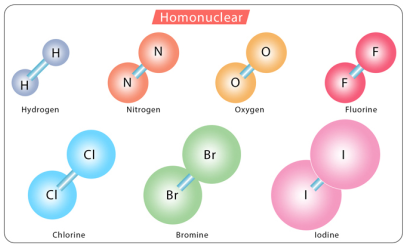
\includegraphics[width=\textwidth]{p2_new_a.png}
        \caption{Ejemplos moléculas diatómicas}
        \label{fig:imagen1}
    \end{subfigure}
    \hspace{0.5cm} % Espacio entre las imágenes
    % Segunda imagen
    \begin{subfigure}[b]{0.3\textwidth}
        \centering
        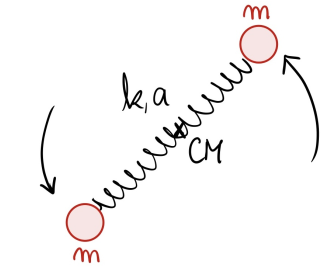
\includegraphics[width=\textwidth]{p2_new_b.png}
        \caption{Modelo simple de una molécula diatómica}
        \label{fig:imagen2}
    \end{subfigure}
    % \caption{Pregunta 3.}
    \label{fig:imagenes}
\end{figure}

\newpage
% \newboxquestion{P3}\\

% Un bloque $B$ de masa $m$ está apoyado en una superficie plana con la cual tiene coeficientes de roce estático y dinámico $\mu _e$ y $μ_d$. El bloque está además unido a un resorte (constante elástica $k$ y largo natural $l_0$) cuyo otro extremo está fijo a la superficie (figura). Inicialmente el resorte está con su largo natural. La superficie se vá inclinando muy lentamente a partir de la posición horizontal ($\alpha = 0$). Siempre es cierto que $\mu _e > \mu _d$

% \begin{enumerate}[label=\alph*)]
%     \item ¿Cuál es el ángulo máximo $\alpha ^*$ antes que el bloque deslice?.
%     \item Suponiendo que cuando $\alpha = \alpha^*$, se deja de mover la superficie plana y el bloque comienza a deslizar, determine el máximo estiramiento del resorte y determine la máxima rapidez que alcanza $B$ durante el movimiento.
%     \item Determine si, una vez alcanzado el estiramiento máximo, $B$ permanece en reposo o si se debiera satisfacer una condición especial para que eso ocurra (propuesto).\\
%     Sol: 
% \end{enumerate}

% \begin{figure}[ht] % [h] indica que se coloca la imagen aquí (here)
%     \centering % Centra la imagen
%     
\includegraphics[width=0.3\textwidth]{P3.png} % Ajusta el tamaño de la imagen
%     \caption{Pregunta 3.} % Subtítulo de la imagen
%     \label{fig:p3} % Etiqueta opcional para referencias
% \end{figure}

\newboxquestion{P4} \textbf{(Propuesto)}\\

Una partícula de masa $m$ se encuentra unida a un extremo de una barra de largo $L$ y masa despreciable. La barra puede rotar en torno al punto fijo $O$ sobre un plano inclinado como se muestra en la figura. El coeficiente de roce cinético entre la partícula y el plano es $\mu$. Se quiere determinar la rapidez mínima que es necesaria dar a la partícula para que ésta realice una vuelta en torno al punto $O$.

\begin{figure}[ht] % [h] indica que se coloca la imagen aquí (here)
    \centering % Centra la imagen
    
\includegraphics[width=0.35\textwidth]{P4.png} % Ajusta el tamaño de la imagen
    \caption{Pregunta 4.} % Subtítulo de la imagen
    \label{fig:p4} % Etiqueta opcional para referencias
\end{figure}

% \newboxquestion{P5}\\ %Muñoz C1 2012-2 con Pauta

% Una argolla de masa $m$ se encuentra inserta en un aro vertical rugoso de radio $R$, unida al extremo de un resorte de constante elástica $k$ y largo natural $l_0= R$, el cual está enrollado a lo largo del aro y cuyo otro extremo está fijo en el punto $A$ como muestra la figura. Los coeficientes de roce estático y cinético entre la argolla y el aro son $\mu e$ y $\mu c$, respectivamente. Determine:

% \begin{enumerate}[label=\alph*)]
%     \item Las constantes $k$ y $\mu _e$ tal que la argolla pueda permanecer en reposo en el rango $\pi /6 \leq \theta \leq \pi/3$.
%     \item La fuerza adicional $\vec{F}= F(\theta)\hat \theta$ que se debe aplicar a la partícula para que ella tenga un movimiento con $\dot \theta = w_0$ constante en el rango $0 \leq \theta \leq \pi$, con $w_0$ constante conocida.

% \end{enumerate}

% \begin{figure}[ht] % [h] indica que se coloca la imagen aquí (here)
%     \centering % Centra la imagen
%     
\includegraphics[width=0.3\textwidth]{p5.png} % Ajusta el tamaño de la imagen
%     \caption{Pregunta 5.} % Subtítulo de la imagen
%     \label{fig:p5} % Etiqueta opcional para referencias
% \end{figure}

% \newboxquestion{P6}\\ %Auxiliar Mono CLaudia torque II

% Se tiene un péndulo con punto fijo en su extremo como en la figura, compuesto por una barra ideal de largo $L = N\epsilon$ que tiene $N$ masas $m$ a intervalos $\epsilon$ en todo su largo de modo que la masa total es $M = Nm$.

% \begin{enumerate}[label=\alph*)]
%     \item Escriba la posición y velocidad de la n-ésima partícula. Con esto, encuentre el momento angular total del sistema. Considere $N \gg 1$.
%     \item Obtenga la ecuación de movimiento del sistema.
%     \item Encuentre $\phi(t)$ cuando $ϕ \ll 1$. Para condiciones iniciales arbitrarias.

% \end{enumerate}

% \begin{figure}[ht] % [h] indica que se coloca la imagen aquí (here)
%     \centering % Centra la imagen
%     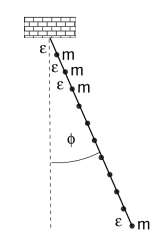
\includegraphics[width=0.2\textwidth]{p6.png} % Ajusta el tamaño de la imagen
%     \caption{Pregunta 6.} % Subtítulo de la imagen
%     \label{fig:p6} % Etiqueta opcional para referencias
% \end{figure}


% FIN DEL DOCUMENTO
\end{document}